\documentclass[12pt,a4paper]{article}

% =========================
% PACKAGES
% =========================
\usepackage[utf8]{inputenc}
\usepackage[T5]{fontenc}
\usepackage[provide=*,vietnamese]{babel}
\usepackage{geometry}
\usepackage{array}
\usepackage{longtable}
\usepackage{booktabs}
\usepackage{multirow}
\usepackage{graphicx}
\usepackage{xcolor}
\usepackage{hyperref}
\usepackage{enumitem}
\usepackage{listings}
\usepackage{fancyhdr}
\usepackage{titlesec}
\usepackage{tabularx}
\usepackage{pgfplots}
\usepackage{tikz}
\usetikzlibrary{shapes.geometric, arrows.meta, positioning, calc}
\pgfplotsset{compat=1.18}

% =========================
% SETTINGS & STYLES
% =========================
\geometry{
    left=2.5cm,
    right=2.5cm,
    top=2.5cm,
    bottom=2.5cm
}

\hypersetup{
    colorlinks=true,
    linkcolor=darkblue,
    urlcolor=darkblue,
    citecolor=darkblue
}

\definecolor{lightgray}{gray}{0.96}
\definecolor{darkblue}{RGB}{0, 70, 140}
\definecolor{darkred}{RGB}{150, 20, 20}
\definecolor{darkgreen}{RGB}{20, 120, 60}
\definecolor{darkorange}{RGB}{210, 110, 20}

\lstdefinestyle{codestyle}{
    backgroundcolor=\color{lightgray},
    basicstyle=\ttfamily\small,
    breaklines=true,
    frame=single,
    columns=fullflexible
}

% Định dạng cho TikZ Diagram
\tikzset{
    box/.style = {rectangle, draw=darkblue, fill=white, thick, text width=3.5cm, align=center, rounded corners, minimum height=1cm},
    widebox/.style = {rectangle, draw=darkblue, fill=white, thick, text width=6.5cm, align=center, rounded corners, minimum height=1cm},
    decision/.style = {diamond, draw=darkred, fill=white, thick, text width=2.5cm, align=center, inner sep=-2pt},
    arrow/.style = {thick, ->, >=stealth},
    line/.style = {thick, -}
}

\pagestyle{fancy}
\fancyhf{}
\lhead{\footnotesize Clinical Ambient Documentation Assistant}
\rhead{\footnotesize Báo cáo Benchmark ASR Lâm sàng}
\cfoot{\thepage}

\titleformat{\section}
{\normalfont\Large\bfseries\color{darkblue}}
{\thesection}{1em}{}

\titleformat{\subsection}
{\normalfont\large\bfseries\color{darkblue}}
{\thesubsection}{1em}{}

\title{
    \textbf{Báo cáo Đánh giá Mô hình ASR Tiếng Việt Lâm sàng}\\
    \large Benchmark, Phân tích Lỗi Y khoa và Khuyến nghị Triển khai\\
    \normalsize Dự án: Local-first Clinical Ambient Documentation Assistant for Vietnamese Outpatient Care
}

\author{Vũ Đức Duy}
\date{Ngày lập: 06/06/2026}

\begin{document}

\maketitle

\begin{abstract}
Báo cáo này tổng hợp kết quả đánh giá các mô hình nhận dạng giọng nói tự động (Automatic Speech Recognition -- ASR) cho bối cảnh ghi chép lâm sàng tiếng Việt. Mục tiêu kỹ thuật của giai đoạn này là xác định mô hình có khả năng đạt Word Error Rate (WER) dưới 20\% trên tập dữ liệu tiếng Việt y khoa, đồng thời đánh giá các lỗi có ý nghĩa an toàn lâm sàng như bỏ sót từ phủ định, sai triệu chứng, sai tên thuốc, sai liều lượng và sai dấu hiệu nguy hiểm.

Kết quả thực nghiệm trên tập phát triển VietMed gồm 200 mẫu cho thấy mô hình \texttt{khanhld/chunkformer-ctc-large-vie} đạt Strict WER và Normalized WER đều ở mức 12.90\%, vượt mục tiêu kỹ thuật $<20\%$. Tuy nhiên, phân tích lỗi y khoa cho thấy không có mô hình nào đạt trạng thái ``zero clinical risk''. Cả ChunkFormer, PhoWhisper-medium và PhoWhisper-base vẫn còn lỗi bỏ sót phủ định hoặc triệu chứng ở một số mẫu, có thể gây đảo nghĩa lâm sàng nếu đưa trực tiếp vào hồ sơ y tế. Vì vậy, báo cáo khuyến nghị sử dụng ChunkFormer làm benchmark độ chính xác, tiếp tục fine-tuning \texttt{vinai/PhoWhisper-medium} làm phương án cân bằng tốc độ--chất lượng, và bắt buộc bổ sung tầng kiểm tra an toàn hậu ASR trước khi nối sang clinical fact extraction và SOAP note generation.
\end{abstract}

\tableofcontents
\newpage

% ======================================================
\section{Tóm tắt Điều hành}

\subsection{Mục tiêu báo cáo}

Báo cáo này được xây dựng nhằm phục vụ trao đổi kỹ thuật với mentor/sếp về kết quả đánh giá ASR trong dự án \textit{Clinical Ambient Documentation Assistant}. Trọng tâm không chỉ là so sánh WER giữa các mô hình, mà còn đánh giá khả năng sử dụng trong một pipeline y tế có yêu cầu truy vết, an toàn và human-in-the-loop.

Các mục tiêu chính gồm:
\begin{itemize}[leftmargin=1.2cm]
    \item So sánh các mô hình ASR tiếng Việt/y khoa trên cùng một tập phát triển VietMed.
    \item Đo Strict WER, Normalized WER, Strict CER và Normalized CER bằng cùng một giao thức chuẩn hóa.
    \item Phân tích các lỗi lâm sàng có rủi ro cao: phủ định, triệu chứng, thuốc, liều/đơn vị, dị ứng và red flag.
    \item Đề xuất mô hình primary, mô hình backup và kế hoạch fine-tuning cho tuần tiếp theo.
\end{itemize}

\subsection{Kết luận nổi bật}

\begin{table}[h]
\centering
\caption{Tóm tắt kết quả điều hành}
\begin{tabularx}{\textwidth}{|l|X|}
\hline
\textbf{Hạng mục} & \textbf{Kết luận} \\
\hline
Mô hình chính xác nhất & \texttt{khanhld/chunkformer-ctc-large-vie}, đạt WER 12.90\%, vượt mục tiêu $<20\%$. \\
\hline
Mô hình thực tiễn nhất & \texttt{vinai/PhoWhisper-medium}, đạt Normalized WER 21.51\%, runtime khoảng 0.42 giây/mẫu. \\
\hline
Mô hình nhẹ nhất & \texttt{vinai/PhoWhisper-base}, runtime khoảng 0.14 giây/mẫu nhưng WER còn cao hơn medium. \\
\hline
Mô hình bị loại khỏi hướng chính & \texttt{openai/whisper-small}, Normalized WER 53.23\%, không cạnh tranh trên tiếng Việt y khoa trong thử nghiệm này. \\
\hline
Rủi ro lâm sàng chính & Tất cả mô hình đều còn lỗi bỏ sót phủ định và triệu chứng; đây là nhóm lỗi có thể đảo nghĩa lâm sàng. \\
\hline
Khuyến nghị trước mắt & Chạy ChunkFormer trên test\_holdout đúng một lần, đồng thời chuẩn bị fine-tuning PhoWhisper-medium và xây tầng kiểm tra an toàn hậu ASR. \\
\hline
\end{tabularx}
\end{table}

\subsection{Thông điệp chính}

Kết quả WER $<20\%$ là điều kiện kỹ thuật cần, nhưng chưa đủ cho hệ thống ghi chép lâm sàng. Một mô hình có WER thấp vẫn có thể không an toàn nếu bỏ sót các từ khóa như ``không'', ``chưa'', ``dị ứng'', ``đau ngực'', ``khó thở'' hoặc sai liều lượng thuốc. Vì vậy, kết quả tuần này nên được hiểu theo hai lớp:
\begin{enumerate}[leftmargin=1.2cm]
    \item \textbf{Lớp ASR Accuracy:} ChunkFormer hiện là mô hình đạt độ chính xác tổng quát tốt nhất.
    \item \textbf{Lớp Clinical Safety:} Cần có hậu kiểm bằng từ điển y khoa, kiểm tra phủ định, kiểm tra số/liều và review của bác sĩ trước khi dùng trong ghi chú lâm sàng.
\end{enumerate}

% ======================================================
\section{Bối cảnh \& Mục tiêu Đánh giá}

\subsection{Bối cảnh dự án}

Dự án hướng đến một trợ lý ghi chép lâm sàng chạy theo định hướng local-first cho bối cảnh khám ngoại trú tiếng Việt. Hệ thống nhận audio cuộc khám, tạo transcript, phân đoạn người nói, trích xuất clinical facts có nguồn dẫn, tạo SOAP-lite draft và đưa cho bác sĩ xác nhận trước khi dữ liệu trở thành bản ghi có giá trị sử dụng.

Trong pipeline này, ASR là tầng đầu tiên. Nếu ASR sai, các tầng phía sau như diarization, clinical fact extraction, source attribution và SOAP note generation đều có nguy cơ sai dây chuyền. Vì vậy, benchmark ASR phải được đánh giá không chỉ bằng WER/CER mà còn bằng lỗi lâm sàng.

\subsection{Mục tiêu định lượng}

Mục tiêu định lượng được đặt ra cho giai đoạn này:
\begin{itemize}[leftmargin=1.2cm]
    \item Đạt WER $<20\%$ trên dữ liệu tiếng Việt y khoa.
    \item Có benchmark tái lập trên cùng một split.
    \item Không sử dụng test\_holdout để chọn mô hình.
    \item Ghi nhận và phân tích các lỗi y khoa quan trọng.
\end{itemize}

Baseline tham chiếu do mentor/sếp cung cấp là Whisper-small fine-tuned trên VietMed với WER khoảng 31\%. Do đó, mô hình được chọn cần cải thiện rõ ràng so với mốc này.

\subsection{Phạm vi đánh giá}

Phạm vi của báo cáo này bao gồm:
\begin{itemize}[leftmargin=1.2cm]
    \item Benchmark trên tập dev VietMed gồm 200 mẫu.
    \item So sánh bốn mô hình: ChunkFormer, PhoWhisper-medium, PhoWhisper-base và Whisper-small.
    \item Phân tích tốc độ suy luận và lỗi y khoa.
    \item Đưa ra quyết định mô hình cho test\_holdout và kế hoạch fine-tuning tuần 4.
\end{itemize}

Báo cáo này chưa bao gồm đánh giá trên dữ liệu bệnh nhân thật, chưa đánh giá full outpatient encounter audio, và chưa đánh giá diarization.

% ======================================================
\section{Dữ liệu, Chia tập và Kiểm soát Benchmark}

\subsection{Nguồn dữ liệu}

Dữ liệu đánh giá chính là VietMed, một nguồn speech y khoa tiếng Việt được sử dụng trong dự án cho mục tiêu benchmark ASR. Trong quá trình thực nghiệm, dữ liệu được đưa vào data lake theo kiến trúc Bronze/Silver/Evaluation:
\begin{itemize}[leftmargin=1.2cm]
    \item \textbf{Bronze:} Raw audio, raw transcript, metadata, license snapshot và checksum.
    \item \textbf{Silver:} Audio đã chuẩn hóa 16kHz mono WAV, manifest ASR, duration và checksum.
    \item \textbf{Evaluation:} test\_holdout cố định, không dùng để huấn luyện hoặc chọn checkpoint.
\end{itemize}

\subsection{Chiến lược chia tập}

Tập VietMed sau khi ingest và chuẩn hóa được chia thành ba phần:

\begin{table}[h]
\centering
\caption{Chiến lược chia tập VietMed}
\begin{tabularx}{\textwidth}{|l|r|X|}
\hline
\textbf{Split} & \textbf{Số mẫu} & \textbf{Mục đích sử dụng} \\
\hline
train\_candidate & 600 & Dùng cho fine-tuning nội bộ, không dùng để báo cáo kết quả cuối. \\
\hline
dev & 200 & Dùng cho model selection, so sánh baseline và chọn checkpoint. \\
\hline
test\_holdout & 200 & Chỉ dùng để xác nhận cuối cùng, không dùng để chọn mô hình. \\
\hline
\end{tabularx}
\end{table}

\subsection{Kiểm tra rò rỉ dữ liệu}

Benchmark chỉ có ý nghĩa khi không có rò rỉ giữa train/dev/test. Theo báo cáo tuần 3, leakage check đạt trạng thái PASS: không có trùng lặp \texttt{sample\_id} giữa ba tập. Đây là điều kiện quan trọng để tránh tình trạng metric ảo.

\subsection{Kiểm soát tính tái lập}

ChunkFormer đã được chạy lại độc lập trên 200 mẫu dev và kết quả WER khớp chính xác với lần chạy trước. Điều này cho thấy pipeline inference, manifest, text normalization và script tính metric có tính ổn định đủ để tiếp tục dùng làm benchmark trong tuần 4.

\begin{figure}[h]
\centering
\resizebox{0.95\textwidth}{!}{
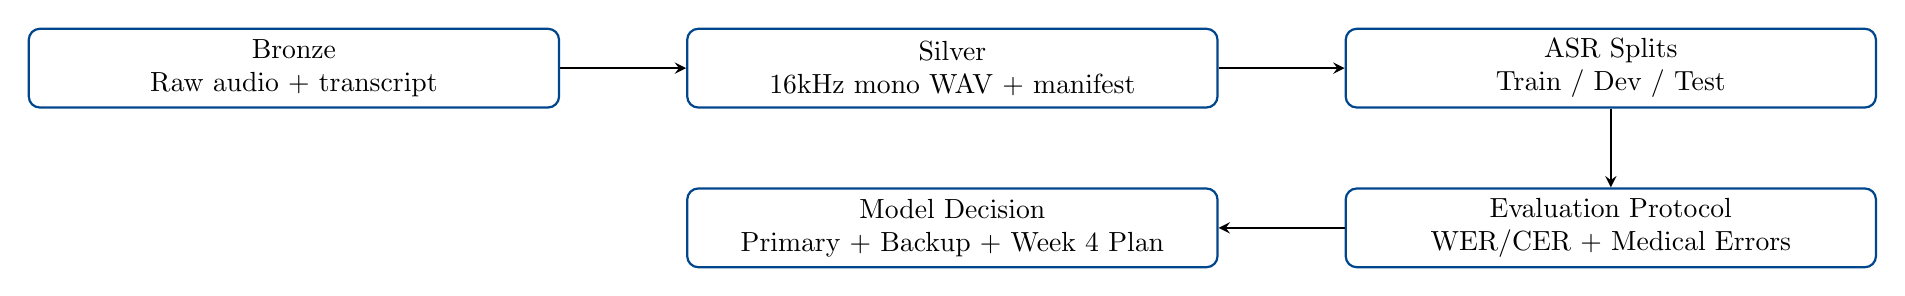
\begin{tikzpicture}[node distance=1cm and 1.6cm]
\node (raw) [widebox] {Bronze\\Raw audio + transcript};
\node (silver) [widebox, right=of raw] {Silver\\16kHz mono WAV + manifest};
\node (split) [widebox, right=of silver] {ASR Splits\\Train / Dev / Test};
\node (eval) [widebox, below=of split] {Evaluation Protocol\\WER/CER + Medical Errors};
\node (report) [widebox, left=of eval] {Model Decision\\Primary + Backup + Week 4 Plan};

\draw [arrow] (raw) -- (silver);
\draw [arrow] (silver) -- (split);
\draw [arrow] (split) -- (eval);
\draw [arrow] (eval) -- (report);
\end{tikzpicture}
}
\caption{Luồng dữ liệu ASR từ Bronze/Silver đến benchmark và quyết định mô hình}
\end{figure}

% ======================================================
\section{Giao thức Đo lường}

\subsection{Các chỉ số chính}

Báo cáo sử dụng bốn chỉ số:
\begin{enumerate}[leftmargin=1.2cm]
    \item \textbf{Strict WER:} So sánh reference và prediction ở dạng nguyên bản.
    \item \textbf{Normalized WER:} So sánh sau chuẩn hóa text.
    \item \textbf{Strict CER:} Character Error Rate nguyên bản.
    \item \textbf{Normalized CER:} Character Error Rate sau chuẩn hóa.
\end{enumerate}

Trong bối cảnh tiếng Việt y khoa, Normalized WER đặc biệt quan trọng vì transcript có thể biểu diễn số và đơn vị theo nhiều cách khác nhau, ví dụ ``năm trăm miligam'' và ``500 mg''.

\subsection{Chuẩn hóa transcript}

Text normalization áp dụng các bước:
\begin{itemize}[leftmargin=1.2cm]
    \item Chuyển lowercase.
    \item Chuẩn hóa Unicode NFC.
    \item Loại bỏ dấu câu không có giá trị y khoa.
    \item Chuẩn hóa khoảng trắng.
    \item Chuẩn hóa một số biểu diễn y khoa như đơn vị và số: \texttt{năm trăm miligam} $\rightarrow$ \texttt{500 mg}, \texttt{ba mươi bảy độ tám} $\rightarrow$ \texttt{37.8 độ}.
\end{itemize}

Điểm quan trọng là cùng một script chuẩn hóa được áp dụng cho mọi mô hình, bảo đảm tính công bằng trong so sánh.

\subsection{Giới hạn của WER trong y tế}

WER là chỉ số cần thiết nhưng không đủ. Hai transcript có cùng WER có thể có mức rủi ro lâm sàng rất khác nhau. Ví dụ:
\begin{itemize}[leftmargin=1.2cm]
    \item Mất từ ``không'' trong câu ``không đau ngực'' có thể đảo nghĩa lâm sàng.
    \item Sai ``500 mg'' thành ``50 mg'' có thể ảnh hưởng nghiêm trọng đến ghi nhận thuốc.
    \item Sai tên bệnh như ``parkinson'' thành cụm từ vô nghĩa làm mất thông tin chẩn đoán.
\end{itemize}

Vì vậy, báo cáo bổ sung phân tích lỗi y khoa theo nhóm rủi ro.

% ======================================================
\section{Các Mô hình được Đánh giá}

\begin{table}[h]
\centering
\caption{Tổng quan các mô hình ASR được đánh giá}
\small
\resizebox{\textwidth}{!}{
\begin{tabular}{|l|l|p{5.5cm}|p{5.5cm}|}
\hline
\textbf{Mô hình} & \textbf{Kiến trúc} & \textbf{Điểm mạnh} & \textbf{Điểm yếu / Lưu ý} \\
\hline
\texttt{chunkformer-ctc-large-vie} & CTC / ChunkFormer & WER thấp nhất; phù hợp làm accuracy benchmark. & Runtime chậm hơn; cần pipeline CTC riêng; cần rà soát license nếu dùng ngoài nội bộ. \\
\hline
\texttt{PhoWhisper-medium} & Seq2Seq / Whisper & Cân bằng tốc độ và chất lượng; phù hợp fine-tuning; runtime tốt. & Zero-shot chưa đạt WER $<20\%$; cần fine-tuning và safety layer. \\
\hline
\texttt{PhoWhisper-base} & Seq2Seq / Whisper & Rất nhanh; phù hợp phương án edge hoặc máy yếu. & WER cao hơn medium; cần đánh đổi chất lượng. \\
\hline
\texttt{whisper-small} & Seq2Seq / Whisper & Baseline quốc tế, dễ chạy. & WER quá cao trong thử nghiệm này; không phù hợp làm hướng chính. \\
\hline
\end{tabular}
}
\end{table}

% ======================================================
\section{Kết quả Benchmark}

\subsection{Bảng kết quả tổng hợp}

\begin{table}[h]
\centering
\caption{Kết quả benchmark trên tập dev VietMed 200 mẫu}
\resizebox{\textwidth}{!}{
\begin{tabular}{|r|l|r|r|r|r|l|}
\hline
\textbf{Rank} & \textbf{Mô hình} & \textbf{Strict WER} & \textbf{Norm. WER} & \textbf{Strict CER} & \textbf{Norm. CER} & \textbf{Runtime} \\
\hline
1 & \texttt{khanhld/chunkformer-ctc-large-vie} & 12.90\% & 12.90\% & 12.03\% & 12.03\% & $\sim$1.23s/mẫu \\
\hline
2 & \texttt{vinai/PhoWhisper-medium} & 24.64\% & 21.51\% & 19.83\% & 19.54\% & $\sim$0.42s/mẫu \\
\hline
3 & \texttt{vinai/PhoWhisper-base} & 26.75\% & 24.11\% & 21.05\% & 20.73\% & $\sim$0.14s/mẫu \\
\hline
4 & \texttt{openai/whisper-small} & 58.58\% & 53.23\% & 46.69\% & 44.85\% & $\sim$0.26s/mẫu \\
\hline
\end{tabular}
}
\end{table}

\subsection{Biểu đồ Normalized WER}

\begin{figure}[h]
\centering
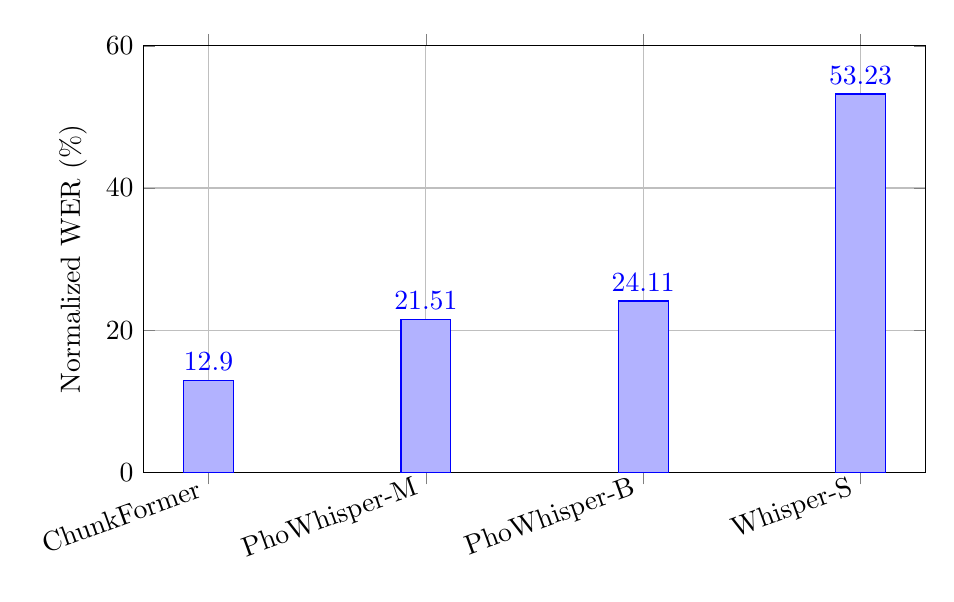
\begin{tikzpicture}
\begin{axis}[
    ybar,
    width=0.95\textwidth,
    height=7cm,
    bar width=18pt,
    ylabel={Normalized WER (\%)},
    symbolic x coords={ChunkFormer,PhoWhisper-M,PhoWhisper-B,Whisper-S},
    xtick=data,
    x tick label style={rotate=20, anchor=east},
    ymin=0,
    ymax=60,
    nodes near coords,
    nodes near coords align={vertical},
    grid=major
]
\addplot coordinates {
    (ChunkFormer,12.90)
    (PhoWhisper-M,21.51)
    (PhoWhisper-B,24.11)
    (Whisper-S,53.23)
};
\end{axis}
\end{tikzpicture}
\caption{So sánh Normalized WER giữa các mô hình ASR}
\end{figure}

\subsection{Nhận định từ kết quả}

\begin{itemize}[leftmargin=1.2cm]
    \item \textbf{ChunkFormer} là mô hình duy nhất đạt mục tiêu WER $<20\%$ trên tập dev. Đây là benchmark độ chính xác tốt nhất hiện tại.
    \item \textbf{PhoWhisper-medium} chưa đạt ngưỡng $<20\%$ ở trạng thái zero-shot, nhưng gần mục tiêu và có tốc độ nhanh hơn đáng kể.
    \item \textbf{PhoWhisper-base} là phương án nhẹ, hữu ích cho edge deployment hoặc máy cấu hình thấp, nhưng cần cải thiện thêm.
    \item \textbf{Whisper-small} không phù hợp làm hướng chính cho tiếng Việt y khoa trong thử nghiệm này.
\end{itemize}

% ======================================================
\section{Phân tích Lỗi Lâm sàng}

\subsection{Taxonomy lỗi y khoa}

Bên cạnh WER/CER, hệ thống phân tích sáu nhóm lỗi có ý nghĩa lâm sàng:

\begin{longtable}{|p{3.2cm}|p{2.6cm}|p{7.5cm}|}
\caption{Phân loại lỗi ASR có rủi ro y khoa}\\
\hline
\textbf{Nhóm lỗi} & \textbf{Mức rủi ro} & \textbf{Ý nghĩa} \\
\hline
\endfirsthead

\hline
\textbf{Nhóm lỗi} & \textbf{Mức rủi ro} & \textbf{Ý nghĩa} \\
\hline
\endhead

Negation & Critical & Bỏ sót hoặc ảo giác từ phủ định có thể đảo nghĩa lâm sàng, ví dụ ``không đau'' thành ``đau''. \\
\hline
Allergy & Critical & Sai hoặc bỏ sót dị ứng có thể gây rủi ro điều trị nghiêm trọng. \\
\hline
Medication & High & Sai tên thuốc ảnh hưởng trực tiếp đến ghi chép điều trị. \\
\hline
Dose/Unit & High & Sai liều hoặc đơn vị có thể gây sai lệch 10 lần hoặc hơn. \\
\hline
Symptom & High & Bỏ sót triệu chứng làm thiếu thông tin chẩn đoán. \\
\hline
Red flag & High & Bỏ sót đau ngực, khó thở, sốt cao hoặc dấu hiệu nguy hiểm làm giảm khả năng phát hiện tình huống cần tái khám/ưu tiên. \\
\hline
\end{longtable}

\subsection{Kết quả lỗi y khoa mở rộng}

\begin{table}[h]
\centering
\caption{Lỗi y khoa trên tập dev, bao gồm ChunkFormer}
\resizebox{\textwidth}{!}{
\begin{tabular}{|l|r|r|r|r|r|r|r|}
\hline
\textbf{Mô hình} & \textbf{Phủ định miss} & \textbf{Triệu chứng miss} & \textbf{Thuốc miss} & \textbf{Liều/đơn vị miss} & \textbf{Dị ứng miss} & \textbf{Red flag miss} & \textbf{Mẫu Critical/High} \\
\hline
ChunkFormer & 7 & 7 & 0 & 1 & 0 & 0 & 7 \\
\hline
PhoWhisper-medium & 7 & 7 & 0 & 1 & 0 & 0 & 7 \\
\hline
PhoWhisper-base & 6 & 9 & 0 & 1 & 0 & 0 & 6 \\
\hline
\end{tabular}
}
\end{table}

\subsection{Ý nghĩa an toàn}

Kết quả trên cho thấy WER thấp không đồng nghĩa với không có lỗi lâm sàng. ChunkFormer có WER tốt nhất, nhưng số mẫu có lỗi Critical/High vẫn tương đương PhoWhisper-medium. Do đó, mô hình ASR không nên được xem là nguồn sự thật cuối cùng. Transcript phải tiếp tục đi qua:
\begin{itemize}[leftmargin=1.2cm]
    \item kiểm tra phủ định;
    \item kiểm tra thuật ngữ y khoa;
    \item kiểm tra thuốc/liều/đơn vị;
    \item kiểm tra red flag;
    \item source attribution;
    \item review của bác sĩ.
\end{itemize}

\subsection{Ví dụ lỗi nguy hiểm}

\begin{table}[h]
\centering
\caption{Ví dụ lỗi lâm sàng từ manual audit}
\resizebox{\textwidth}{!}{
\begin{tabular}{|p{3.2cm}|p{4.2cm}|p{4.2cm}|p{3.2cm}|}
\hline
\textbf{Loại lỗi} & \textbf{Reference} & \textbf{Prediction} & \textbf{Rủi ro} \\
\hline
Bỏ sót phủ định & ta \textbf{không} nên sờ nắn bóp vào đấy & ta nên sờ nắn bóp vào đấy & Đảo nghĩa khuyến cáo y khoa \\
\hline
Bỏ sót phủ định & đau đớn thế nào thì bây giờ nó \textbf{không} & mất từ ``không'' & Đảo nghĩa tình trạng đau \\
\hline
Ảo giác phủ định & với cột sống ngực đâu bởi vì & \textbf{không} phải là cổ sống lưng & Tự thêm phủ định, làm sai nghĩa \\
\hline
Sai thuật ngữ bệnh & người bệnh \textbf{parkinson} & người bệnh \textbf{bạc kinh doanh} & Mất thông tin bệnh lý \\
\hline
\end{tabular}
}
\end{table}

% ======================================================
\section{Đánh đổi Tốc độ và Độ chính xác}

\subsection{So sánh thực tiễn}

\begin{table}[h]
\centering
\caption{Đánh đổi giữa Normalized WER và Runtime}
\begin{tabularx}{\textwidth}{|l|r|l|X|}
\hline
\textbf{Mô hình} & \textbf{Norm. WER} & \textbf{Runtime} & \textbf{Phù hợp cho} \\
\hline
ChunkFormer & 12.90\% & $\sim$1.23s/mẫu & Offline batch, accuracy benchmark, safety-critical transcription có hậu kiểm. \\
\hline
PhoWhisper-medium & 21.51\% & $\sim$0.42s/mẫu & Interactive assistant, candidate fine-tuning, near-real-time. \\
\hline
PhoWhisper-base & 24.11\% & $\sim$0.14s/mẫu & Edge/mobile hoặc máy yếu, chấp nhận WER cao hơn. \\
\hline
\end{tabularx}
\end{table}

\subsection{Ma trận khuyến nghị theo kịch bản}

\begin{longtable}{|p{4.2cm}|p{4.2cm}|p{6cm}|}
\caption{Khuyến nghị mô hình theo kịch bản sử dụng}\\
\hline
\textbf{Kịch bản} & \textbf{Mô hình khuyến nghị} & \textbf{Lý do} \\
\hline
\endfirsthead

\hline
\textbf{Kịch bản} & \textbf{Mô hình khuyến nghị} & \textbf{Lý do} \\
\hline
\endhead

Batch transcription/offline & ChunkFormer & Chính xác nhất, runtime chậm hơn nhưng vẫn chấp nhận được nếu không cần realtime. \\
\hline
Interactive clinical assistant & PhoWhisper-medium sau fine-tuning & Tốc độ tốt hơn ChunkFormer, có khả năng đạt target sau adaptation. \\
\hline
Edge hoặc thiết bị hạn chế tài nguyên & PhoWhisper-base & Runtime thấp nhất, phù hợp thử nghiệm thiết bị cấu hình thấp. \\
\hline
Safety-critical documentation & ChunkFormer + HITL review & WER thấp nhất nhưng vẫn phải có bác sĩ kiểm tra. \\
\hline
Fine-tuning tuần 4 & PhoWhisper-medium & Cân bằng tốc độ--chất lượng, kiến trúc Seq2Seq thuận lợi cho adaptation. \\
\hline
\end{longtable}

% ======================================================
\section{Quyết định Mô hình và Kế hoạch Tiếp theo}

\subsection{Quyết định mô hình}

\begin{table}[h]
\centering
\caption{Quyết định mô hình sau benchmark}
\begin{tabularx}{\textwidth}{|l|X|}
\hline
\textbf{Vai trò} & \textbf{Mô hình / Quyết định} \\
\hline
Primary accuracy benchmark & \texttt{khanhld/chunkformer-ctc-large-vie} \\
\hline
Candidate fine-tuning & \texttt{vinai/PhoWhisper-medium} \\
\hline
Fallback edge candidate & \texttt{vinai/PhoWhisper-base} \\
\hline
Model bị loại khỏi hướng chính & \texttt{openai/whisper-small} \\
\hline
\end{tabularx}
\end{table}

\subsection{Kế hoạch hành động ngay}

\begin{enumerate}[leftmargin=1.2cm]
    \item Chạy ChunkFormer trên \texttt{test\_holdout} đúng một lần duy nhất để xác nhận kết quả ngoài dev.
    \item Tính Strict WER, Normalized WER, Strict CER, Normalized CER trên test\_holdout.
    \item Chạy phân tích lỗi y khoa trên kết quả test.
    \item Chuẩn bị fine-tuning PhoWhisper-medium trong tuần 4.
    \item Xây tầng post-ASR clinical safety checker cho phủ định, thuốc/liều, dị ứng và red flag.
    \item Bảo toàn test\_holdout: không dùng để chọn mô hình hoặc điều chỉnh normalization.
\end{enumerate}

\subsection{Chiến lược tuần 4}

Tuần 4 nên tập trung vào hai nhánh:
\begin{itemize}[leftmargin=1.2cm]
    \item \textbf{Nhánh 1 -- Xác nhận ChunkFormer:} Chạy test\_holdout và lập model card cho mô hình primary.
    \item \textbf{Nhánh 2 -- Fine-tuning PhoWhisper-medium:} Dùng train\_candidate 600 mẫu, dev 200 mẫu để giảm Normalized WER và giảm lỗi phủ định/thuốc/liều.
\end{itemize}

Nếu PhoWhisper-medium sau fine-tuning đạt WER $<20\%$ và có lỗi y khoa không tệ hơn ChunkFormer, mô hình này có thể trở thành lựa chọn thực tiễn cho interactive assistant nhờ runtime tốt hơn.

% ======================================================
\section{Rủi ro, Giới hạn và Biện pháp Giảm thiểu}

\subsection{Rủi ro chính}

\begin{longtable}{|p{3.5cm}|p{4.2cm}|p{6cm}|}
\caption{Rủi ro còn lại sau benchmark ASR}\\
\hline
\textbf{Rủi ro} & \textbf{Tác động} & \textbf{Biện pháp giảm thiểu} \\
\hline
\endfirsthead

\hline
\textbf{Rủi ro} & \textbf{Tác động} & \textbf{Biện pháp giảm thiểu} \\
\hline
\endhead

Bỏ sót phủ định & Đảo nghĩa lâm sàng, ví dụ không đau thành đau. & Negation checker, highlight trong UI, bác sĩ xác nhận. \\
\hline
Sai thuật ngữ bệnh/triệu chứng & Mất thông tin lâm sàng quan trọng. & Từ điển y khoa, keyword recall, post-ASR flagging. \\
\hline
Sai thuốc/liều/đơn vị & Có thể ảnh hưởng nội dung ghi nhận điều trị. & Regex số/liều, double-check UI, cảnh báo bắt buộc. \\
\hline
WER thấp nhưng safety chưa đạt & Metric kỹ thuật gây cảm giác an toàn giả. & Báo cáo song song WER và clinical error metrics. \\
\hline
Test leakage & Làm kết quả benchmark mất giá trị. & Test chỉ chạy cho selected model, không dùng test để chọn checkpoint. \\
\hline
Domain gap & VietMed chưa đại diện đầy đủ outpatient encounter thật. & Tạo volunteer/actor data và synthetic audio ở các tuần sau. \\
\hline
License/deployment risk & Một số model có thể không phù hợp thương mại. & Rà soát license trước pilot/commercial. \\
\hline
\end{longtable}

\subsection{Giới hạn của báo cáo}

\begin{itemize}[leftmargin=1.2cm]
    \item Benchmark hiện dựa trên tập dev VietMed, chưa phải test\_holdout cuối cùng.
    \item Chưa có dữ liệu bệnh nhân thật và chưa đánh giá trong điều kiện phòng khám thật.
    \item Chưa đánh giá diarization, speaker role và clinical attribution trên audio thật.
    \item Synthetic outpatient cases hiện phục vụ downstream clinical NLP và safety seed, chưa thay thế được medical speech benchmark.
\end{itemize}

% ======================================================
\section{Kết luận}

Kết quả benchmark cho thấy bài toán đạt WER $<20\%$ là khả thi với mô hình \texttt{khanhld/chunkformer-ctc-large-vie}, khi mô hình này đạt 12.90\% trên tập dev VietMed 200 mẫu. Tuy nhiên, yêu cầu của hệ thống ghi chép lâm sàng không dừng ở WER. Lỗi phủ định, lỗi triệu chứng, lỗi thuốc/liều và lỗi dị ứng vẫn phải được xem là rủi ro cấp cao.

Khuyến nghị triển khai là sử dụng ChunkFormer làm mô hình benchmark độ chính xác trong ngắn hạn, đồng thời fine-tune PhoWhisper-medium như một hướng cân bằng giữa tốc độ, khả năng triển khai và chất lượng. Mọi output ASR cần đi qua lớp kiểm tra an toàn hậu xử lý và bác sĩ xác nhận trước khi được dùng cho clinical fact extraction hoặc SOAP note generation.

% ======================================================
\section{Phụ lục — Giả định}

\begin{enumerate}[leftmargin=1.2cm]
    \item Tất cả số liệu WER/CER được lấy từ kết quả thực nghiệm trong repository dự án.
    \item Runtime được ghi nhận trong môi trường GPU T4 hoặc môi trường tương đương, nên có thể thay đổi khi triển khai local.
    \item Tập dev được dùng cho model selection; test\_holdout chưa được dùng để điều chỉnh mô hình.
    \item Phân tích lỗi y khoa dựa trên từ điển kiểm tra hiện có, chưa thay thế được review của bác sĩ.
\end{enumerate}

\end{document}
